% paper_writing/main.tex
% Target venue: Discover Networks (Springer, open access, ISSN 3004-9792)
%
% TODO-TEMPLATE: replace preamble with sn-jnl.cls before submission.
% The official Springer Nature `sn-jnl` template could not be downloaded in
% this environment (springernature.com template zip returned 404, no CTAN
% package named sn-jnl, GitHub mirror not found). This fallback preamble
% uses a standard article class configured to match sn-jnl's citation style
% (numbered, via natbib) so the draft is compilable. Swap in the real
% sn-jnl.cls and its bibliography style (e.g. sn-mathphys-num.bst) at
% submission time.
\documentclass[11pt]{article}

\usepackage[margin=1in]{geometry}
\usepackage{natbib}
\usepackage{graphicx}
\usepackage{booktabs}
\usepackage{amsmath}
\usepackage{subcaption}
\usepackage{hyperref}

\graphicspath{{figures/}}

\title{Detecting Network Anomalies in Named Data Networking Through Isolation Forest-Based Behavioral Analysis}

\author{
  Ankit Pokhrel \and
  Asmit Phuyal \and
  Darshan Kumar Paudyal \and
  Babu R. Dawadi\thanks{Corresponding author.} \\[1ex]
  Department of Electronics \& Computer Engineering, \\
  Pulchowk Campus, Institute of Engineering, \\
  Tribhuvan University, Lalitpur, Nepal
}

\date{}

\begin{document}

\maketitle

% Abstract — drafted in Task 4
\begin{abstract}
Named Data Networking (NDN) replaces host-centric communication with content-centric named data retrieval, but its in-network caching and stateful forwarding expose routers to Interest Flooding Attacks (IFA) and Cache Pollution (CP) that evade conventional threshold-based detection. This paper presents a single unsupervised Isolation Forest detector, trained only on clean traffic, evaluated on two platforms across the same three topologies (tree, dumbbell, and DFN mesh): miniNDN, an emulation platform running the real NDN Forwarding Daemon, and ndnSIM, an ns-3 simulator. On miniNDN, the detector identifies the IFA attacker node at 91.2\,\%, 98.7\,\%, and 96.8\,\% across the three topologies, at a false-positive rate below 4.3\,\%, and confirms that PIT-based features are non-discriminating, correcting the textbook expectation of PIT exhaustion. Because CP leaves no usable signature in the emulation feature set, an attacker-rate sweep of 297 runs on ndnSIM locates each attack's detection floor, the minimum attacker rate at which reliable detection is sustained at a realistic 1--2\,\% false-positive rate. The sweep's central result: the two floors are an order of magnitude apart and topology-invariant, with CP, a volumetric attack, detected down to approximately 44\,Hz, and IFA, whose signature is qualitative rather than volumetric, detected down to approximately 1.8\,Hz. These findings indicate that the security-relevant limit on unsupervised NDN anomaly detection is not raw model accuracy but a mechanism-dependent detection floor set by how volumetric or qualitative each attack's traffic signature is.
\end{abstract}

\noindent\textbf{Keywords:} Named Data Networking; Interest Flooding Attack; Cache Pollution; Isolation Forest; anomaly detection; detection floor

% Introduction — drafted in Task N

% Related Work — drafted in Task N

% Method
\section{Methodology}
\label{sec:method}

\subsection{Platforms and Topologies}

The detector is evaluated identically on two complementary platforms viz. miniNDN and ndnSIM. \textbf{miniNDN} \cite{cabral2013mini} is an NDN network emulator built on Mininet that runs the real NDN Forwarding Daemon (NFD) inside isolated Linux network namespaces; because the forwarding stack is the genuine production code, counters collected from miniNDN carry real OS scheduling jitter, NFD buffering, and polling artifacts that a purely simulated environment cannot reproduce. \textbf{ndnSIM} \cite{mastorakis2015ndnsim} is an ns-3-based simulator that implements the NDN forwarding pipeline in software; it trades some of miniNDN's realism for deterministic, per-second ground truth and the throughput needed to run the multi-hundred-run attacker-rate sweep on which this paper's central result depends. Running the same detector, unmodified, on both platforms lets the emulation study establish how a real forwarding daemon behaves under attack, while the simulation study reuses that feature-engineering philosophy at a scale emulation cannot support.

Both platforms share the same three topologies (Figure~\ref{fig:topologies}), so any difference observed between IFA and CP, or between platforms, can be attributed to the attack and the forwarding stack rather than to an inconsistent network shape. The \textbf{tree} topology has a single root router, modelling campus or enterprise networks in which traffic flows from consumer leaves through backbone routers to producer leaves. The \textbf{dumbbell} topology connects two stub networks through a shared bottleneck core, modelling wide-area configurations that concentrate PIT pressure at a small number of core routers during a traffic surge. The \textbf{DFN} topology is an irregular mesh derived from the Deutsches Forschungsnetz graph, with heterogeneous node degree and redundant paths, testing whether detection generalizes to a real-world network structure. All three topologies contain nine to twelve nodes on both platforms, with every node type, consumer, producer, and transit router, represented in the collected data.

The two platforms run on different software stacks (Table~\ref{tab:software}). miniNDN runs on Ubuntu 22.04 with NFD and NLSR 22.12; consumer request rates vary between 40 and 80 Interests per second with natural Gaussian variance over a Zipf-distributed catalog, and counters are polled every 3 seconds. ndnSIM runs ndnSIM 2.x on ns-3.35 inside an Ubuntu 20.04 container, with tracer output collected every 1 second; each consumer issues a Zipf-Mandelbrot request process over a fixed catalog sized so the cache stays useful and the background traffic remains live throughout the run. Despite the differing polling intervals and traffic generators, both platforms feed the same downstream feature-engineering and detection pipeline.

\begin{table}[t]
\centering
\caption{Software environment.}
\label{tab:software}
\begin{tabular}{@{}lll@{}}
\toprule
\textbf{Component}        & \textbf{Tool / Library}   & \textbf{Version}  \\
\midrule
NDN emulation             & miniNDN                   & 0.4.0             \\
NDN simulation            & ndnSIM on ns-3            & 2.x / ns-3.35     \\
NDN forwarding daemon     & NFD                       & 22.12             \\
Name-based routing        & NLSR                      & 22.12             \\
Machine learning          & scikit-learn              & 1.4+              \\
Data processing           & pandas, numpy             & latest stable     \\
Model persistence         & joblib                    & latest stable     \\
Runtime                   & Python                    & 3.10+             \\
\bottomrule
\end{tabular}
\end{table}

\subsection{Feature Engineering}
\label{sec:features}

On miniNDN, ten behavioral features listed in Table~\ref{tab:features} are computed per node per interval from NFD counter deltas and absolute state values, drawn from two lightweight commands, \textit{nfdc status} and \textit{nfdc cs info}. The set deliberately retains \textit{pit\_size} and \textit{pit\_growth\_rate}: PIT exhaustion is the textbook signature of IFA, so keeping these two lets the emulation study test directly whether that signature survives contact with a real forwarding daemon's polling behaviour, rather than assuming it in advance. On ndnSIM, nine face-level features are derived instead from the simulator's tracers: three rates, \textit{in\_interests\_rate}, \textit{out\_interests\_rate}, and \textit{in\_data\_rate}, and six ratios, \textit{cache\_hit\_ratio}, \textit{satisfaction\_ratio}, \textit{timeout\_ratio}, \textit{nack\_ratio}, \textit{interest\_amp} ($=\Delta\text{Out}/\Delta\text{In}$), and \textit{data\_ratio} ($=\Delta\text{InData}/\Delta\text{In}$). No PIT-derived feature is included in the ndnSIM set, a choice informed by the emulation-stage result that PIT counters do not discriminate attack from normal traffic at practical polling intervals.

\begin{table}[t]
\centering
\caption{The ten miniNDN behavioral features.}
\label{tab:features}
\begin{tabular}{@{}lll@{}}
\toprule
\textbf{Feature}              & \textbf{Definition}                                                       & \textbf{Category} \\
\midrule
\textit{pit\_size}            & $\textit{nPitEntries}$ (absolute)                                         & State \\
\textit{pit\_growth\_rate}    & $\Delta\textit{nPitEntries} / \Delta t$                                   & Rate  \\
\textit{cs\_size}             & $\textit{nCsEntries}$ (absolute)                                          & State \\
\textit{cache\_hit\_ratio}    & $\textit{nHits} / (\textit{nHits} + \textit{nMisses})$                    & Ratio \\
\textit{satisfaction\_ratio}  & $\textit{nSat} / (\textit{nSat} + \textit{nUnsat})$                       & Ratio \\
\textit{unsatisfied\_ratio}   & $\textit{nUnsat} / (\textit{nSat} + \textit{nUnsat})$                     & Ratio \\
\textit{in\_interests\_rate}  & $\Delta\textit{nInInterests} / \Delta t$                                  & Rate  \\
\textit{out\_interests\_rate} & $\Delta\textit{nOutInterests} / \Delta t$                                 & Rate  \\
\textit{in\_data\_rate}       & $\Delta\textit{nInData} / \Delta t$                                       & Rate  \\
\textit{nack\_rate}           & $\Delta(\textit{nInNacks} + \textit{nOutNacks}) / \Delta t$               & Rate  \\
\bottomrule
\end{tabular}
\end{table}

All ratio features are set to zero when both numerator and denominator are zero, which happens during idle intervals in which a node forwarded no traffic; without this rule an idle interval records an artificial satisfaction ratio of zero and teaches the model that failure is normal, which measurably collapses attacker detection. Rate features are separately clipped to the [1st, 99th] percentile range computed on normal training data, to keep outliers from distorting the StandardScaler fit described below. \textit{nack\_rate} and \textit{pit\_growth\_rate} are the exception: both are identically zero throughout normal traffic, so their normal-data percentile range has zero width, and clipping them would clip away the entire attack-time signal before it reaches the model. These two features are therefore never clipped, on either platform.

Absolute rate features carry a further caveat: they are load-dependent, so a normal run collected at a higher request rate than the training data can be false-flagged purely by the load difference. A ratio-only variant of the feature set (satisfaction ratio, cache-hit ratio, NACK rate, data-to-interest ratio, and forwarding ratio) is therefore evaluated separately as a load-invariant alternative. Both variants are trained on identical clean normal traffic and compared on held-out normal captures collected at heavier legitimate load and on the IFA attack captures. As shown in Figure~\ref{fig:load-fpr}, on the heaviest-load normal capture, which carries roughly twice the training interest rate, the full absolute-rate set false-flags about 41\,\% of benign intervals, whereas the ratio-only set holds its false-positive rate near 2\,\%, close to its training level; on a second higher-load normal capture the two sit at 4.9\,\% and 1.3\,\%. This reduction in load-induced false positives, roughly twentyfold on the heaviest-load run, comes at no cost to detection: as Figure~\ref{fig:load-detection} shows, pooled over the affected nodes of the attack captures, IFA detection is retained at 71\,\% for the ratio-only set against 64\,\% for the absolute-rate set. The ratio-only variant does, however, shift detection away from the high-rate attacker node itself toward the downstream victims and routers whose satisfaction collapses, since it no longer keys on raw interest volume. This load robustness is why ratio features dominate the ndnSIM set, whose six ratios were carried over directly from this comparison.

\begin{figure}[t]
\centering
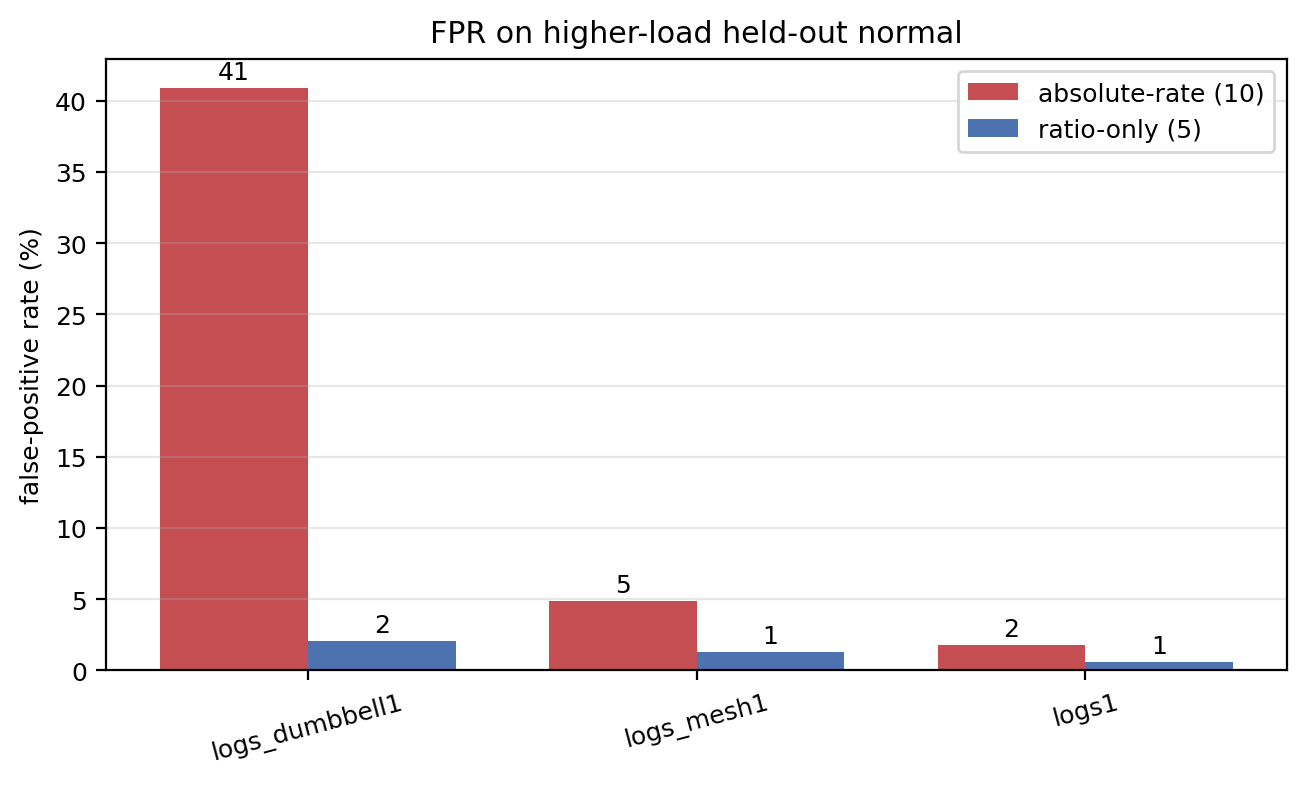
\includegraphics[width=0.6\textwidth]{fig_load_fpr}
\caption{False-positive rate on higher-load held-out normal captures. The absolute-rate set spikes to $\sim$41\,\% on the heaviest-load run (\textit{logs\_dumbbell1}, roughly twice the training interest rate), while the ratio-only set stays near 2\,\%. Both detectors are trained on the same clean normal traffic; every flagged interval here is a false positive.}
\label{fig:load-fpr}
\end{figure}

\begin{figure}[t]
\centering
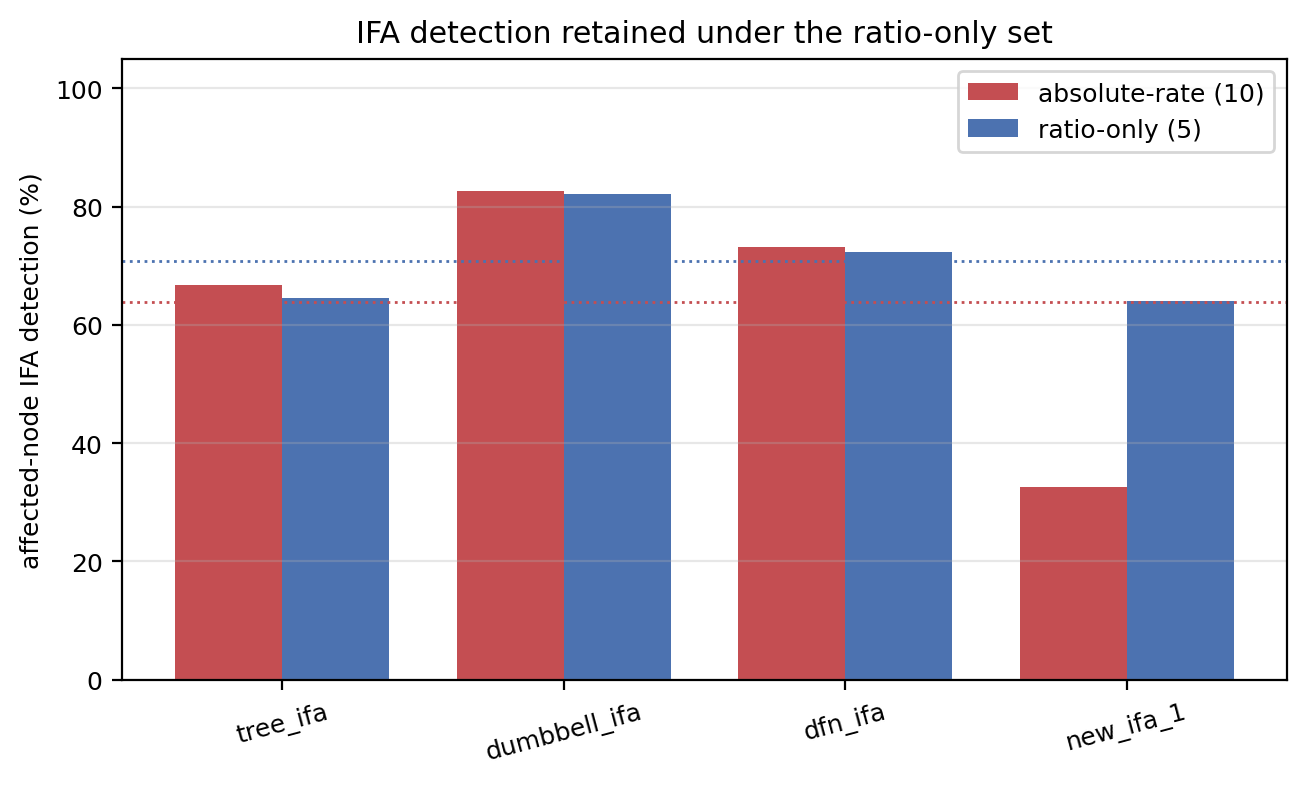
\includegraphics[width=0.6\textwidth]{fig_load_detection}
\caption{Affected-node IFA detection under each feature set. The false-positive reduction of Figure~\ref{fig:load-fpr} costs no detection: the ratio-only set retains attack detection (dotted lines mark the per-set means, 71\,\% ratio-only versus 64\,\% absolute-rate).}
\label{fig:load-detection}
\end{figure}

\subsection{Isolation Forest Pipeline}

Both feature sets feed the same two-step scikit-learn pipeline. A StandardScaler first normalizes every feature to zero mean and unit variance, so that features of very different magnitude, an absolute PIT count against a bounded ratio, contribute comparably to the anomaly score, and an IsolationForest is then fitted on the scaled output. The forest uses 200 isolation trees, a contamination parameter of 0.01, and a fixed random seed for reproducibility, and it is fitted exclusively on normal traffic: no labelled attack sample is ever seen during training. A single global model is trained per platform on the combined clean data pooled across all three topologies, rather than one model per topology, so the reported detection rates reflect a detector not tuned to any one network shape.

Isolation Forest \cite{liu2008isolation, liu2012isolation} detects anomalies structurally rather than statistically. Each tree recursively partitions the feature space through random feature selection and random split values until every point is isolated in its own leaf; because anomalous points are few and different from the bulk of normal traffic, they are isolated in fewer splits, giving them a shorter path length on average. For an instance $x$ scored against an ensemble of trees built over $n$ training samples, the anomaly score is given by Equation~\eqref{eq:iforest},

\begin{equation}
\label{eq:iforest}
s(x, n) = 2^{-\dfrac{E[h(x)]}{c(n)}}
\end{equation}

\noindent where $E[h(x)]$ is the mean path length of $x$ across all trees and $c(n)$, defined in Equation~\eqref{eq:cn},

\begin{equation}
\label{eq:cn}
c(n) = 2H(n-1) - \frac{2(n-1)}{n}, \qquad H(i) = \ln(i) + 0.5772,
\end{equation}

\noindent is the expected path length of an unsuccessful search in a binary search tree, normalizing $s$ against training-set size. In Equation~\eqref{eq:iforest} a score near 1 indicates a strong anomaly; a score near 0.5 is characteristic of normal instances. scikit-learn's \textit{decision\_function} reports a shifted, signed variant in which more negative values denote greater anomaly strength, and it is this signed score, not the raw $s(x,n)$ of Equation~\eqref{eq:iforest}, that the threshold calibration below operates on.

\subsection{Threshold Calibration and Score Normalization}

Rather than hand-tuning a fixed cutoff, the anomaly decision boundary $\theta$ is derived from the training score distribution itself: $\theta$ is set so that approximately 1\,\% of normal training samples fall on its anomalous side, consistent with the contamination parameter, which places $\theta$ at a raw \textit{decision\_function} value of $0.0$ (positive scores normal, negative anomalous). The fitted pipeline, $\theta$, the training score range $[s_{\min}, s_{\max}]$, and the feature column ordering are serialised together, so scoring at evaluation time is fully determined by the training run.

For reporting and alerting, raw \textit{decision\_function} scores are mapped by Equation~\eqref{eq:norm} onto a 0--100 scale that anchors $\theta$ at 30, $s_{\max}$ at 100, and $s_{\min}$ at 0:

\begin{equation}
\label{eq:norm}
\hat{s} =
\begin{cases}
30 + \dfrac{s - \theta}{s_{\max} - \theta} \times 70 & \text{if } s \ge \theta \\[8pt]
\dfrac{30 \times (s - s_{\min})}{\theta - s_{\min}} & \text{if } s < \theta,
\end{cases}
\end{equation}

\noindent clipped to $[0, 100]$. Two thresholds on the scale of Equation~\eqref{eq:norm} are used throughout the evaluation. The \textbf{strict threshold (30\,\%)} corresponds exactly to the raw auto-calibrated boundary $\theta = 0.0$; a normalized score below it indicates a confident anomaly. The \textbf{operational threshold (50\,\%)} is a lower-sensitivity level that also catches samples whose raw score lies slightly above $\theta$ but whose position on the normalized scale still signals a deviation; it matters most for IFA, whose signature depresses the raw score only moderately, so reading the strict threshold alone would under-report it.

\subsection{Detection-Floor Definition}
\label{sec:floor-def}

Reporting detection accuracy at a single attack rate says nothing about how an attacker who throttles down evades the detector, so this paper defines detection reliability as a function of attacker rate rather than as a single number. Let $D(r)$ denote the pooled detection rate (recall) over every attacker-labelled sample collected at attacker rate $r$, aggregated across all three topologies and every replicate seed run at that rate. Given the ordered set $R$ of attacker rates sampled by the rate sweep, the \textbf{detection floor} $r^{*}$ is the smallest sampled rate at and above which pooled detection never again drops below a 90\,\% reliability bar. It is defined formally in Equation~\eqref{eq:floor}:

\begin{equation}
\label{eq:floor}
r^{*} = \min\left\{\, r_i \in R \;:\; D(r_j) \ge 0.90 \text{ for all } r_j \in R,\ r_j \ge r_i \,\right\}.
\end{equation}

where, $r^{*}$ is an empirical quantity, not a closed-form threshold: it is measured, separately for each attack, by evaluating $D(r)$ at every sweep rate and locating the point below which reliable detection is no longer sustained. An attacker below $r^{*}$ escapes reliable detection at the false-positive rate the sweep otherwise holds; one above it does not. This definition is applied to both IFA and CP in the simulation study, where the two resulting floors differ by an order of magnitude, a difference this paper attributes to whether the attack's signature is volumetric or qualitative.

\subsection{Evaluation Metrics}

Detection performance on labelled test data is quantified with two threshold-dependent quantities, computed at both the 30\,\% and 50\,\% normalized-score thresholds and, on the simulation platform, pooled per attacker rate to obtain the $D(r)$ used in Equation~\eqref{eq:floor}. Both are given in Equation~\eqref{eq:DetRate}:

\begin{equation}
\label{eq:DetRate}
\text{Detection Rate} = \frac{TP}{TP + FN}, \qquad
\text{FPR} = \frac{FP}{FP + TN}.
\end{equation}

Statistical separability between attack-time and normal-time score distributions, independent of where any threshold is drawn, is assessed with the two-sample Kolmogorov--Smirnov test. Its $D$-statistic is the maximum absolute distance between the two empirical cumulative distribution functions,

\begin{equation}
\label{eq:ks}
D = \sup_{x} \left| F_{\text{normal}}(x) - F_{\text{attack}}(x) \right|,
\end{equation}

A larger $D$ in Equation~\eqref{eq:ks} indicates the two distributions are more separable, regardless of threshold placement. The detection rate and FPR of Equation~\eqref{eq:DetRate} and the KS $D$-statistic of Equation~\eqref{eq:ks} are reported together throughout, since a detector can score well on one while masking a weakness the others expose.

% Emulation
\section{Emulation Study: Interest Flooding on miniNDN}
\label{sec:emulation}

The emulation study runs the global Isolation Forest detector described in Section~\ref{sec:method} against Interest Flooding on miniNDN's real NFD forwarding stack. Attacker node c1 floods each topology with Interests for names that do not resolve, so every request it issues is destined to time out rather than be satisfied; the detector never sees a labelled attack sample during training, and the same model, trained once on pooled clean traffic from all three topologies, is evaluated unmodified against tree, dumbbell, and DFN. Because the attack, the traffic model, and the polling interval are all fixed by the real NFD forwarding stack rather than by a simulator's approximation of it, this study is where the paper's assumptions about IFA's behavioral signature are first tested against genuine forwarding-daemon dynamics, before a much larger set of attacker rates is swept on the simulation platform.

\subsection{Detection and False-Positive Rate}

On held-out normal traffic the global model's false-positive rate stays low at both operating points (Table~\ref{tab:emu-fpr}): at the strict 30\,\% threshold it never exceeds 1.00\,\%, and even at the more permissive operational 50\,\% threshold it stays under 4.3\,\% in every topology. Figure~\ref{fig:emu_score_dist} shows why: the normal and IFA anomaly-score distributions are cleanly separated in all three topologies, with normal traffic concentrated near the high-score end of the scale and attacker traffic pushed toward the anomalous region well before either threshold is reached.

\begin{table}[t]
\centering
\caption{Normal-traffic false-positive rate, global model (attacker-labelled intervals flagged on clean data).}
\label{tab:emu-fpr}
\begin{tabular}{@{}lccc@{}}
\toprule
\textbf{Threshold} & \textbf{Tree} & \textbf{Dumbbell} & \textbf{DFN} \\
\midrule
@30\,\% (strict)       & 0.19\,\% & 1.00\,\% & 0.64\,\% \\
@50\,\% (operational)  & 1.08\,\% & 4.27\,\% & 4.10\,\% \\
\bottomrule
\end{tabular}
\end{table}

\begin{figure}[t]
    \centering
    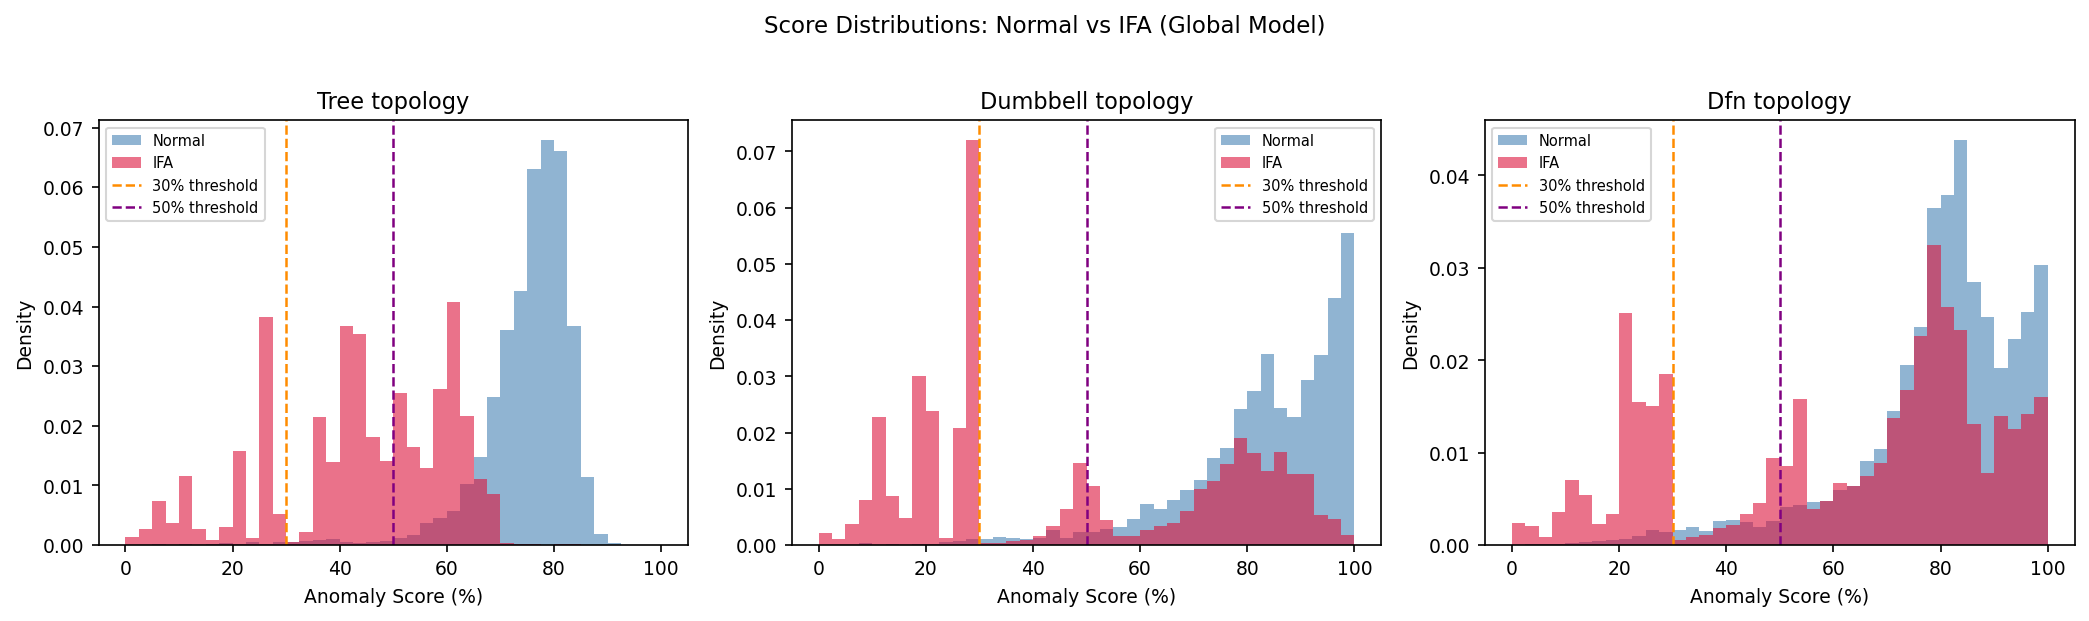
\includegraphics[width=\textwidth]{emu_score_dist}
    \caption{Normal versus IFA normalized anomaly-score distributions for the three topologies (global model). Normal traffic concentrates in the high-score (normal) region while IFA traffic shifts toward the anomalous region, crossing the 30\,\% and 50\,\% thresholds.}
    \label{fig:emu_score_dist}
\end{figure}

Against this low false-positive floor, attacker c1 is detected at high rates in every topology, without any topology-specific retraining (Table~\ref{tab:emu-attacker-det}). Detection is weakest in the tree, where it still exceeds 89\,\% at the strict threshold, and strongest in the dumbbell, where it reaches 98.5\,\%. The gap between the strict and operational thresholds is narrow throughout, indicating that most attacker windows are scored well past the strict boundary rather than clustering just beyond it.

\begin{table}[t]
\centering
\caption{Attacker node c1 detection rate, global model.}
\label{tab:emu-attacker-det}
\begin{tabular}{@{}lcc@{}}
\toprule
\textbf{Topology} & \textbf{Detection @30\,\%} & \textbf{Detection @50\,\%} \\
\midrule
Tree     & 89.1\,\% & 91.2\,\% \\
Dumbbell & 98.5\,\% & 98.7\,\% \\
DFN      & 96.7\,\% & 96.8\,\% \\
\bottomrule
\end{tabular}
\end{table}

\subsection{Per-Node Spatial Fingerprint}

Because the detector operates independently at every node, it does not merely flag c1; it traces the shape of the attack across the network. Figure~\ref{fig:emu_pernode} shows the per-node detection rate in each topology. Backbone and other on-path routers, the nodes that must carry c1's flood toward its unreachable destinations, are flagged at 90--99\,\%, essentially matching the attacker itself, while nodes on branches the flood never reaches stay close to their normal-traffic baseline. The on-path producer p1, which lies at the end of c1's forwarding path in every topology, is flagged as high as 90.5\,\%, whereas the off-path producer p2 remains near baseline throughout. This on-path/off-path split holds cleanly in the dumbbell and DFN topologies, where redundant paths let unaffected branches carry traffic unperturbed.

Table~\ref{tab:emu-spatial} breaks this pattern out per topology at the operational threshold. In the tree, backbone routers r1--r2 sit at 90--90.4\,\%, while the off-path leaf routers r3--r4 fall to 18--22\,\%, and producer p1 clears 90.5\,\% against p2's 30.0\,\%. The dumbbell shows the sharpest contrast: every on-path router, including the bottleneck, sits at 98.7\,\%, while the single off-path router r4 drops to 2.0\,\% and the off-path producer p2 to 2.2\,\%. DFN falls in between, with the on-path core routers r1--r2 at 97\,\% against the off-path edge routers r3--r4 at 7.7--8.8\,\%. In every topology, detection rate at a router or producer tracks whether that node sits on c1's forwarding path, not how close it is to the attacker in hop count; the anomaly score is, in effect, a map of the attack's reach through the network, recovered without any access to routing tables.

\begin{table}[t]
\centering
\caption{Spatial propagation of IFA detection (@50\,\%, global model).}
\label{tab:emu-spatial}
\begin{tabular}{@{}llc@{}}
\toprule
\textbf{Topology} & \textbf{Node group (role)} & \textbf{Detection @50\,\%} \\
\midrule
Tree     & r1, r2 (backbone, on-path)      & 90--90.4\,\% \\
Tree     & r3, r4 (leaf, off-path)         & 18--22\,\% \\
Tree     & p1 / p2 (on-path / off-path producer) & 90.5\,\% / 30.0\,\% \\
Dumbbell & r1, r2, r3, bottleneck (on-path) & 98.7\,\% \\
Dumbbell & r4 (off-path)                    & 2.0\,\% \\
Dumbbell & p1 / p2                          & 72.4\,\% / 2.2\,\% \\
DFN      & r1, r2 (core, on-path)           & 97\,\% \\
DFN      & r3, r4 (edge, off-path)          & 7.7--8.8\,\% \\
DFN      & p1 / p2                          & 46.5\,\% / 2.3\,\% \\
\bottomrule
\end{tabular}
\end{table}

\begin{figure}[t]
    \centering
    \begin{subfigure}{0.32\textwidth}
        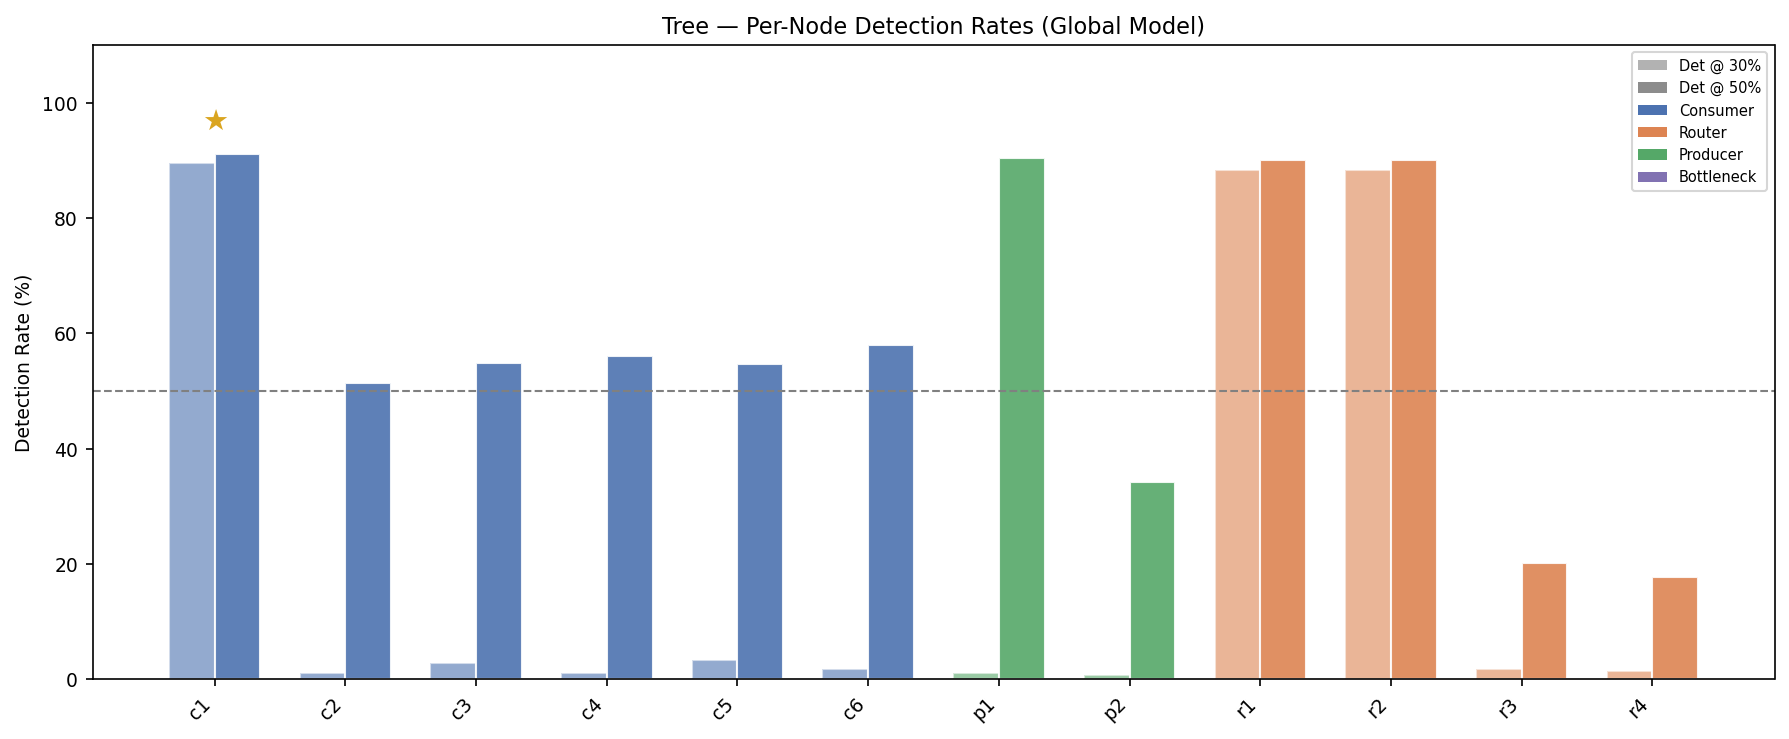
\includegraphics[width=\linewidth]{emu_pernode_tree}
        \caption{Tree}
    \end{subfigure}\hfill
    \begin{subfigure}{0.32\textwidth}
        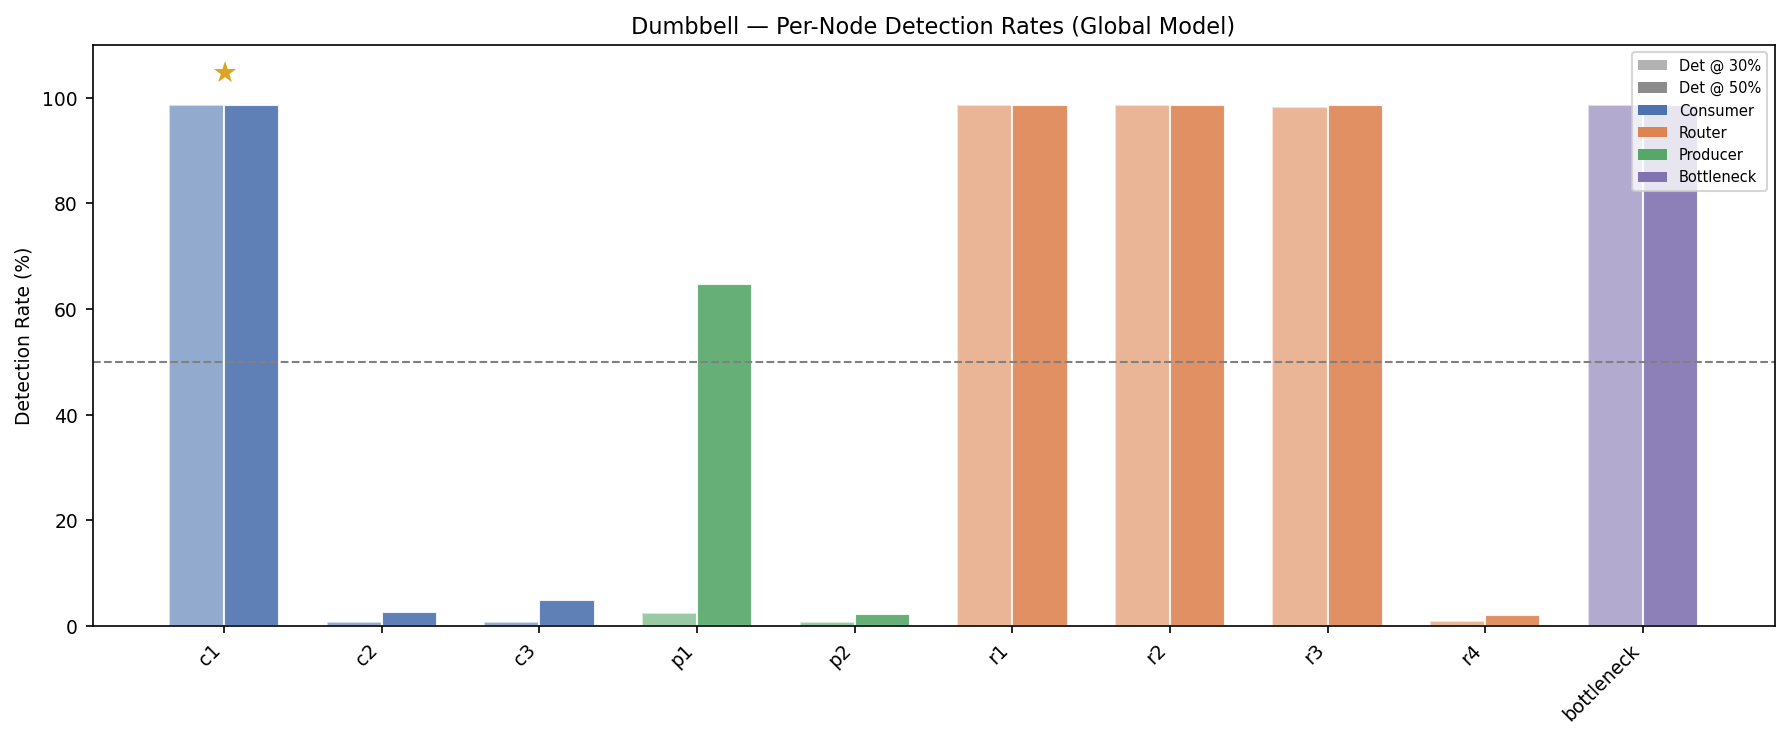
\includegraphics[width=\linewidth]{emu_pernode_dumbbell}
        \caption{Dumbbell}
    \end{subfigure}\hfill
    \begin{subfigure}{0.32\textwidth}
        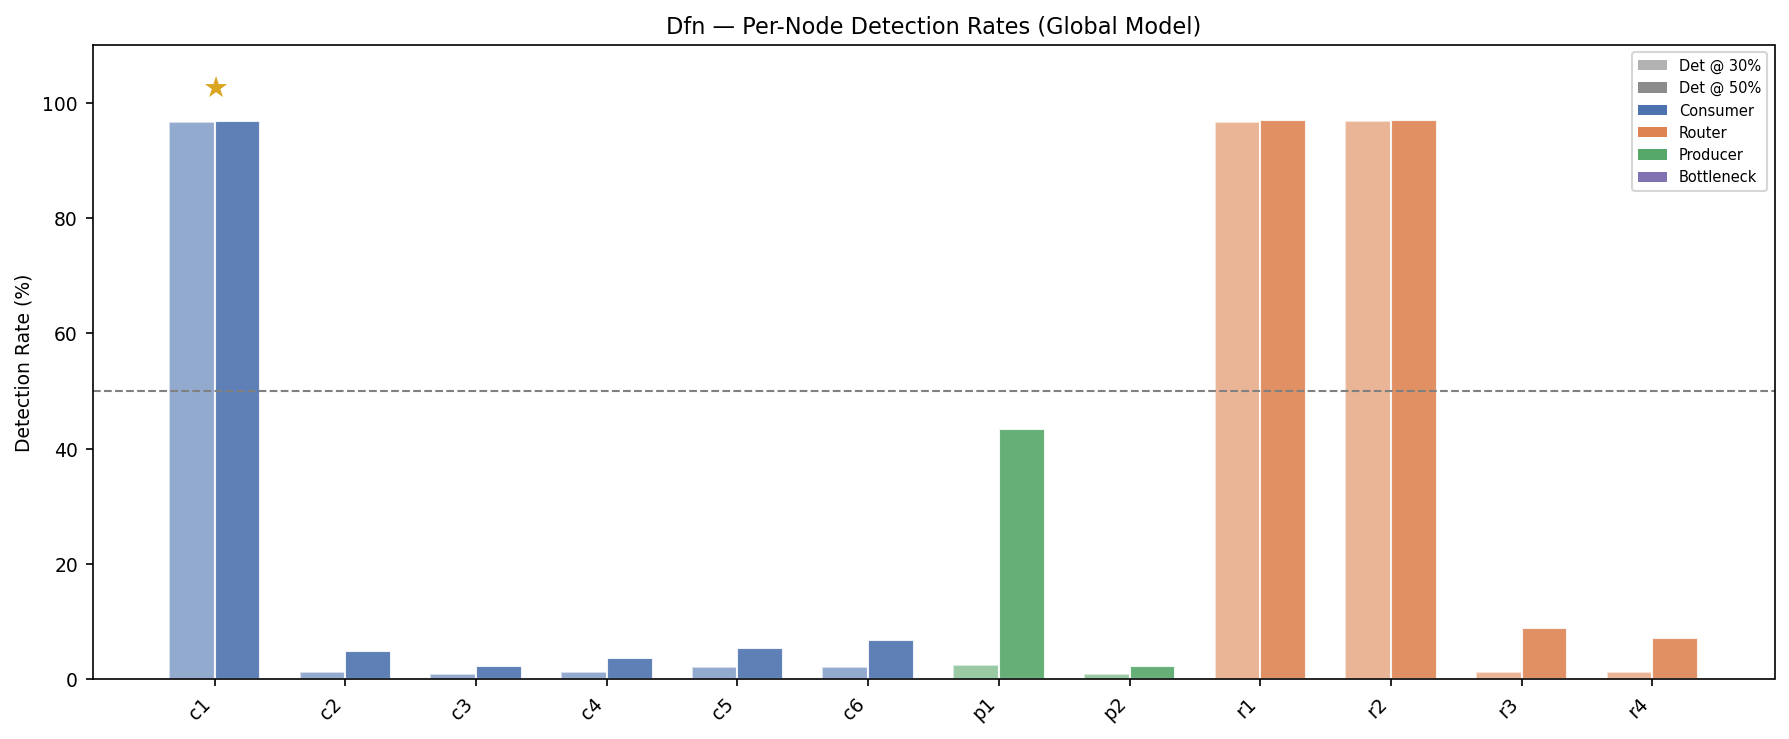
\includegraphics[width=\linewidth]{emu_pernode_dfn}
        \caption{DFN}
    \end{subfigure}
    \caption{Per-node IFA detection rate (global model) for the three topologies. The attacker and on-path routers and producers are strongly detected; off-path nodes remain low, except in the Tree topology, where the flood reaches every branch.}
    \label{fig:emu_pernode}
\end{figure}

The tree topology is the exception, and it is informative rather than a failure. Because every consumer's traffic funnels through the same shared backbone routers r1--r2 before reaching a producer, c1's flood saturates that shared infrastructure and generates NACKs that propagate outward to branches c1 never directly touches. Benign consumers c2--c6 are consequently elevated to 51--58\,\% detection at the operational threshold, an order of magnitude above their dumbbell and DFN counterparts. This is a genuine network effect, not a detector artifact: in a hierarchical topology with a single shared core, IFA degrades service quality network-wide rather than remaining a point attack confined to the flooded consumer's own path, and the per-node detection pattern in Figure~\ref{fig:emu_pernode} captures that spillover correctly rather than over-flagging.

\subsection{The PIT-Feature Myth}
\label{sec:pit-myth}

The feature set retains \textit{pit\_size} and \textit{pit\_growth\_rate} specifically to test the textbook expectation that IFA manifests as PIT exhaustion (Section~\ref{sec:features}). Under the emulation traffic model, that expectation does not hold. Table~\ref{tab:emu-ks} reports the Kolmogorov--Smirnov $D$-statistic, averaged across topologies, between the attacker's normal-time and attack-time distribution for each feature: \textit{pit\_size} separates attack from normal with a mean $D$ of only 0.096, and \textit{pit\_growth\_rate} manages just 0.028, both far below the level needed for a feature to carry usable signal. At NFD's 3-second polling interval, PIT entries fill and drain between successive polls, so the sustained PIT buildup the textbook signature assumes never becomes an observable, persistent counter value; whatever exhaustion occurs is transient and invisible to interval-sampled monitoring.

\begin{table}[t]
\centering
\caption{KS D-statistic for the attacker node c1 (normal vs.\ IFA), by feature, averaged across topologies.}
\label{tab:emu-ks}
\begin{tabular}{@{}lc@{}}
\toprule
\textbf{Feature} & \textbf{Mean $D$} \\
\midrule
satisfaction\_ratio  & 0.947 \\
unsatisfied\_ratio   & 0.947 \\
cache\_hit\_ratio    & 0.939 \\
in\_interests\_rate  & 0.941 \\
nack\_rate           & 0.929 \\
in\_data\_rate       & 0.899 \\
cs\_size             & 0.893 \\
pit\_size            & 0.096 \\
pit\_growth\_rate    & 0.028 \\
\bottomrule
\end{tabular}
\end{table}

The features that do the discriminating are the ones the PIT-exhaustion narrative treats as secondary: satisfaction ratio, cache-hit ratio, and NACK rate all separate attack from normal almost perfectly ($D > 0.9$, $p < 10^{-200}$), a pattern that holds at the attacker and propagates, attenuated, to the on-path routers and producer identified in Figure~\ref{fig:emu_pernode}. Figure~\ref{fig:emu_ks_heatmap_tree} shows this separability broken out node by feature for the tree topology: the attacker and on-path nodes light up on satisfaction, NACK, and cache-hit features while the PIT columns stay uniformly flat, including at the attacker itself. Figure~\ref{fig:emu_feature_importance} corroborates the same conclusion from a different angle, permutation-based feature importance on the fitted model: satisfaction-, NACK-, and cache-hit-derived features dominate the ranking while the PIT-based features contribute negligibly. Together the KS test and the permutation importance correct the PIT-exhaustion assumption directly rather than by omission, which is why the feature set carries satisfaction ratio, cache-hit ratio, and NACK rate as its primary discriminators rather than any PIT-derived count.

\begin{figure}[t]
    \centering
    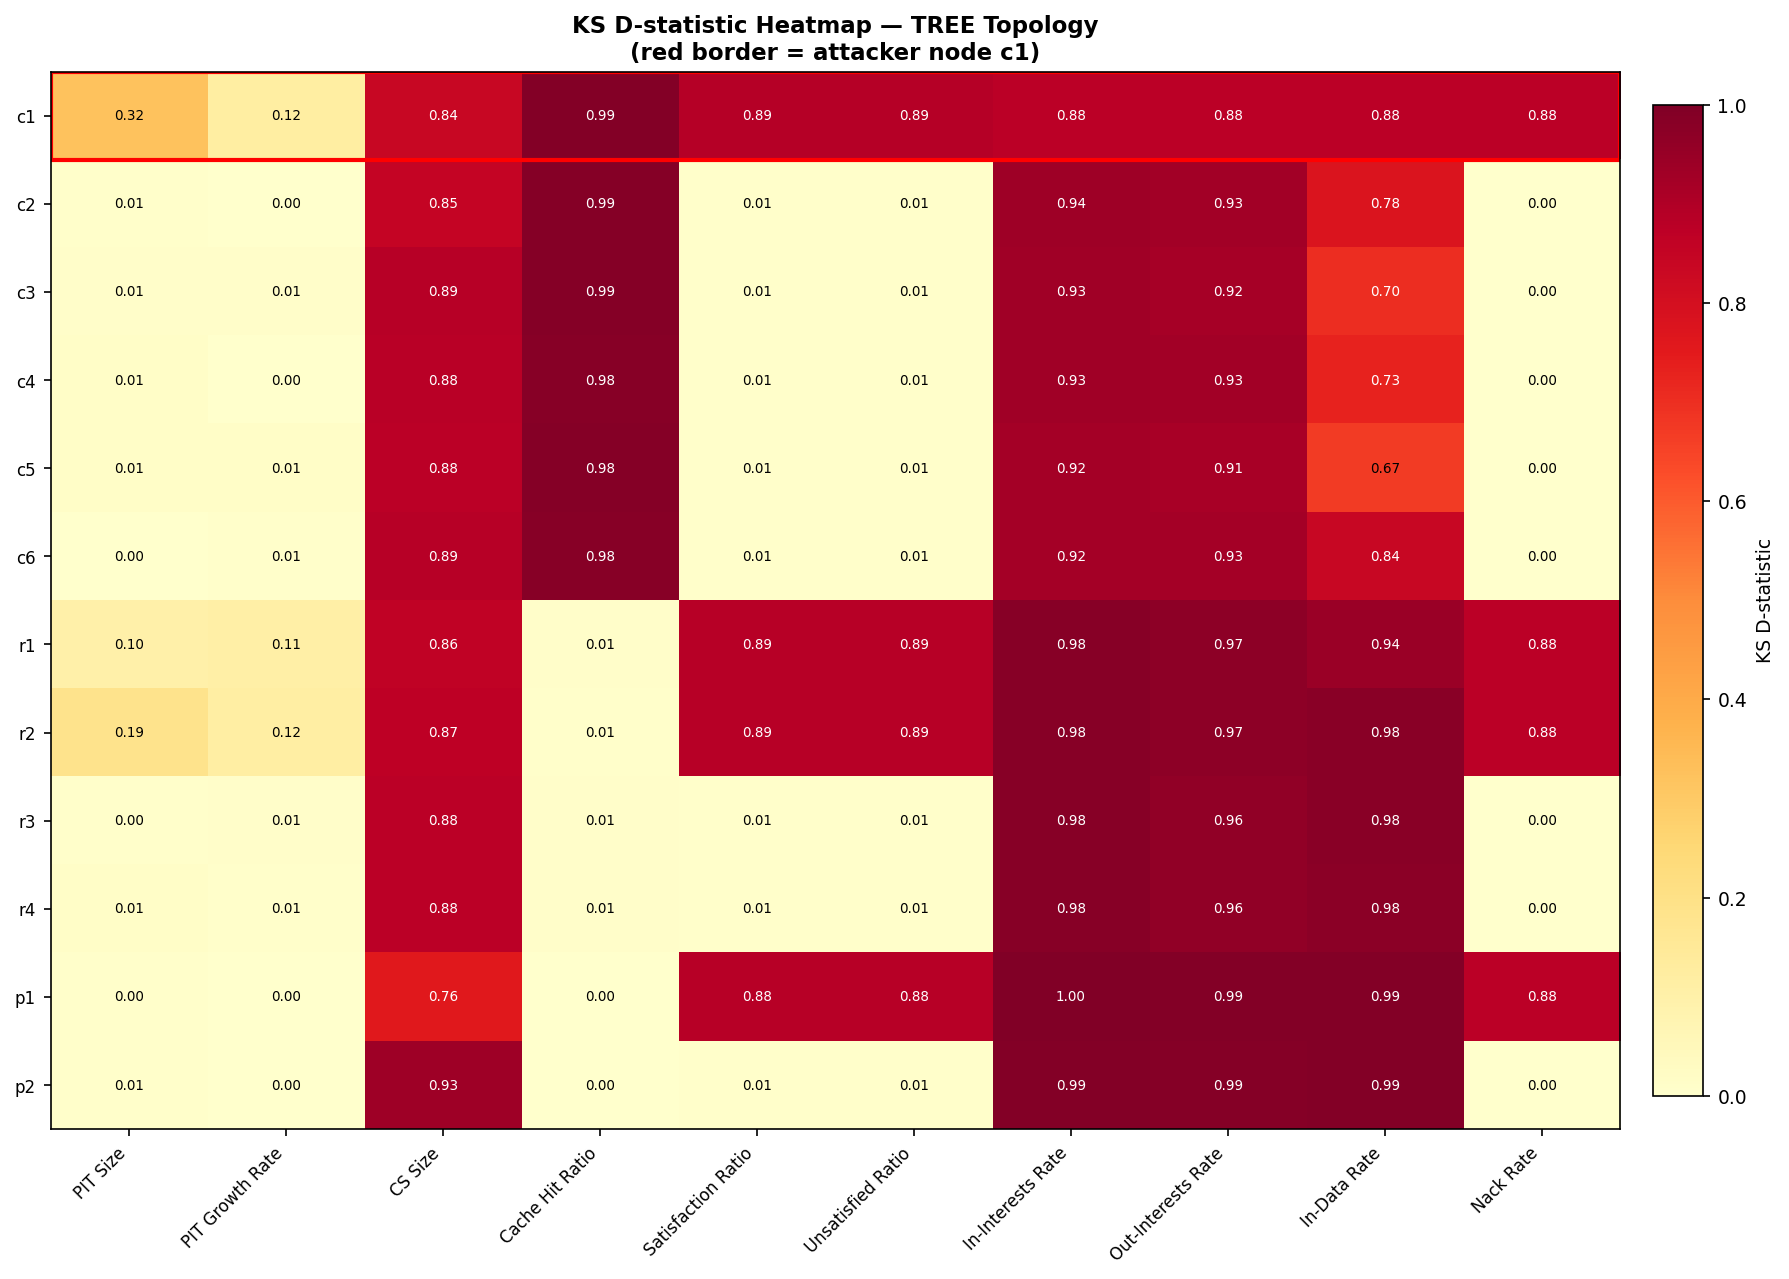
\includegraphics[width=\textwidth]{emu_ks_heatmap_tree}
    \caption{KS D-statistic heatmap (Tree), node by feature. Satisfaction, NACK, and cache-hit features separate the attacker and on-path nodes; PIT features are uniformly non-discriminating.}
    \label{fig:emu_ks_heatmap_tree}
\end{figure}

\begin{figure}[t]
    \centering
    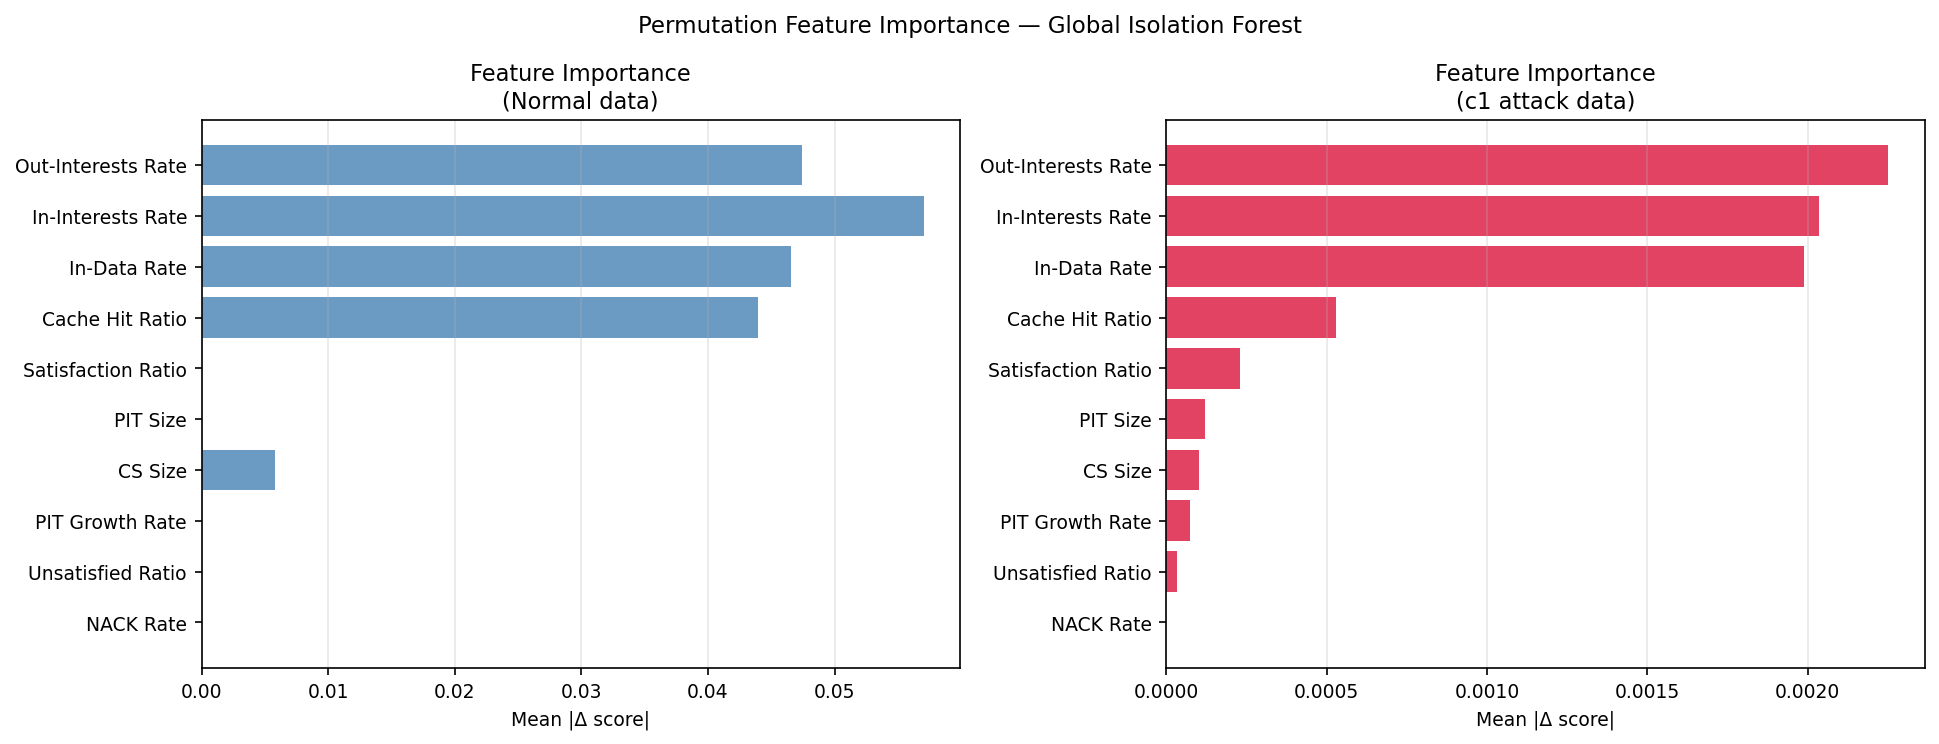
\includegraphics[width=0.82\textwidth]{emu_feature_importance}
    \caption{Permutation-based feature importance on the IFA data (global model). Satisfaction-, NACK-, and cache-hit-derived features dominate; PIT-based features contribute negligibly.}
    \label{fig:emu_feature_importance}
\end{figure}

\subsection{Cache Pollution: A Negative Result}

Cache Pollution was also run against the miniNDN emulation, and it produced no usable behavioral signature. CP's entire mechanism is to lower the cache-hit ratio by requesting unpopular content that evicts entries a legitimate population would otherwise reuse, but under the emulation traffic model the baseline cache-hit ratio at consumer nodes is already close to zero: there is essentially nothing left for the attack to degrade. The satisfaction ratio, the feature set's other strong discriminator, offers no help either, since polluted Interests are still answered by producers and so the ratio stays high throughout the attack. The result is a detector with nothing distinctive to key on: CP-time feature distributions in this setup are statistically indistinguishable from normal traffic.

This negative result is itself a finding, not a dead end. It shows that detecting Cache Pollution behaviorally requires an environment in which the cache is doing meaningful work in the first place, so that pollution has something to visibly disrupt. The miniNDN traffic model does not provide that environment; the ndnSIM simulation study, with its larger catalog and an active, useful cache baseline, does, and it is there that Cache Pollution's detectability is properly characterized.

% Simulation
\section{Simulation Study: Locating the Detection Floor}
\label{sec:simulation}

Cache Pollution left no usable behavioral footprint on miniNDN: the emulation traffic model's cache-hit ratio was already close to zero at consumer nodes, so CP had nothing visible left to degrade, and its requests were still answered, so the satisfaction ratio stayed high throughout the attack (Section~\ref{sec:emulation}). That negative result is not a dead end but a diagnosis, it identifies exactly the environment CP needs to be evaluated honestly: a cache that is doing meaningful work in the first place. ndnSIM~\cite{mastorakis2015ndnsim} supplies that environment, and it supplies something else the emulation platform cannot: the throughput to run hundreds of runs at a swept attacker rate. This section reuses the same global Isolation Forest, the same feature-engineering philosophy, and the same three topologies from Section~\ref{sec:method}, but asks a different question of them. Rather than reporting detection at one attack intensity, it sweeps the attacker rate down until detection breaks, and locates, separately for IFA and CP, the detection floor defined in Equation~\ref{eq:floor}: the lowest attacker rate at which the detector still holds 90\,\% reliability against live background traffic.

\subsection{Setup and the Attacker-Rate Sweep}

Every scenario runs for 600\,s. Attacks inject at $t = 300$\,s, splitting each run into a 300\,s normal segment and a 300\,s attack segment, and the detector is fit on the first 200\,s of normal traffic only, so no attack-time sample is ever seen during training. All scenario types share an identical legitimate background, so the only difference between a normal run and an attack run is the attack itself: every consumer runs a Zipf-Mandelbrot request process at 10 interests/s over a catalog of $N = 300$ distinct names. The catalog size is not incidental. An earlier, smaller catalog exhausted the request stream about 30\,s into each run, after which the consumers fell silent and the background died; a model trained on that traffic learns that ``normal'' means an idle network, and every subsequent detection number is measured against silence rather than against a working system. At $N = 300$ the legitimate consumers keep emitting at roughly 4.4 interests/s each for the full 600\,s, including through the attack window, while the cache stays useful enough for CP to have something to pollute (Figure~\ref{fig:traffic-health}). Every result reported below is measured against this live, unbroken background.

\begin{figure}[t]
    \centering
    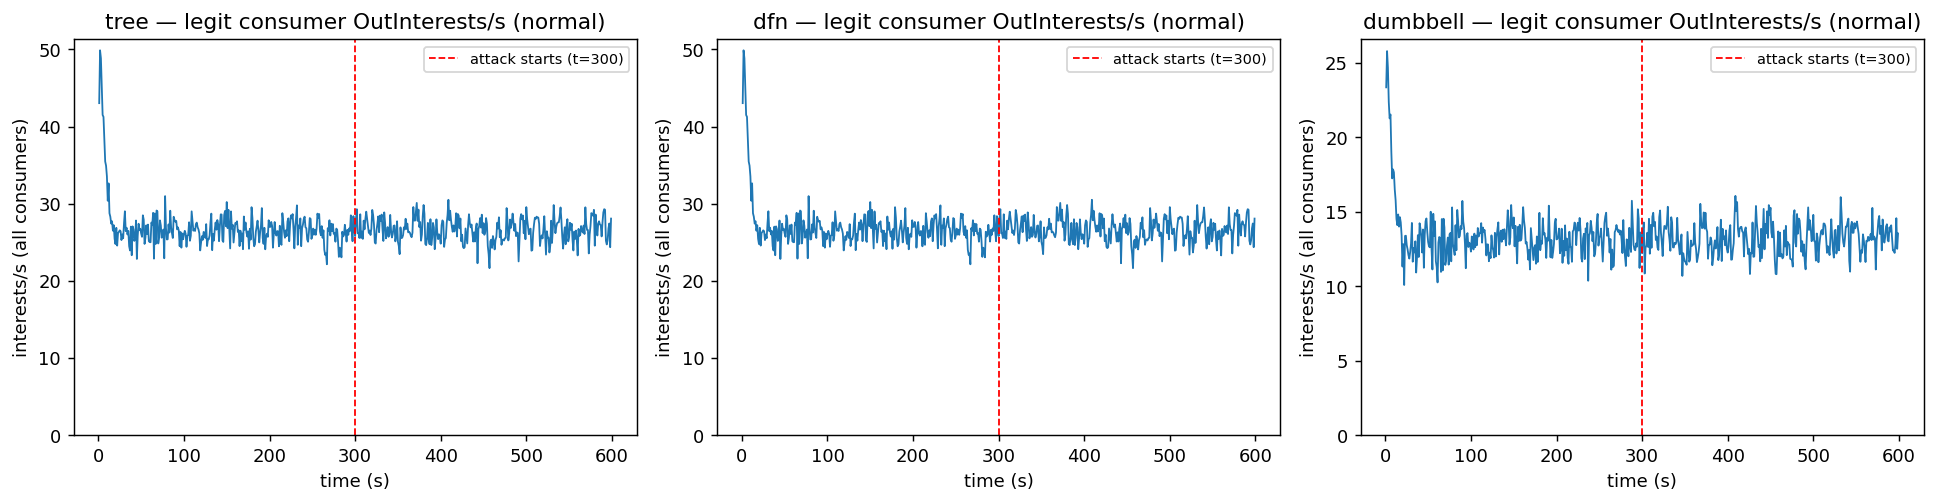
\includegraphics[width=0.75\textwidth]{fig_legit_traffic_health}
    \caption{Legitimate consumer interest rate over time (ndnSIM), attack window shaded. The background stays flat and active for the full 600\,s, so detection is measured against a busy network rather than a silent one.}
    \label{fig:traffic-health}
\end{figure}

The two attacks exercise the two data structures the introduction identifies as NDN's attack surface, in as pure a form as the simulator allows. In the \textbf{IFA} scenario, the attacker launches four concurrent constant-bit-rate Interest streams, in a fixed 40:30:20:10 rate ratio scaled to the chosen total rate, toward a \textit{/evil} namespace served by a co-located black-hole producer that registers the prefix but never returns Data. Every attacker Interest is therefore destined to time out, generating genuine PIT pressure, timeouts, and NACKs rather than a simulator artifact. In the \textbf{CP} scenario, two attacker consumers each request 50 distinct junk names under \textit{/ndn/junk/} at a combined rate scaled to the sweep point; because the junk namespace is served, producers answer every request, so the junk Data enters router Content Stores through ordinary caching and evicts entries a legitimate population would otherwise have reused, raising the legitimate cache-miss rate. The name diversity is held fixed across the sweep, so only the per-name request frequency changes with rate.

To locate each floor precisely, the attacker rate is swept and replicated over seeds, sampled densely where each attack's own floor is expected to lie (Table~\ref{tab:sim-sweep}). Every configuration runs on all three topologies, giving \textbf{297 runs} in total: 15 normal, 156 IFA, and 126 CP, each emitting per-second ground-truth labels alongside the tracer output described in Section~\ref{sec:method}.

\begin{table}[t]
\centering
\caption{ndnSIM attacker-rate sweep. Floor-region rates use five seeds; the two highest rates are single-seed anchors. Rates are per attacker (CP has two attackers).}
\label{tab:sim-sweep}
\begin{tabular}{@{}lll@{}}
\toprule
\textbf{Scenario} & \textbf{Attacker rates (interests/s)} & \textbf{Seeds} \\
\midrule
Normal & (no attack) & 1--5 \\
\midrule
\multirow{2}{*}{IFA}
  & 1, 2, 4, 6, 8, 10, 12, 15, 20, 30 & 1--5 \\
  & 50, 100 & 1 (anchor) \\
\midrule
\multirow{2}{*}{CP}
  & 10, 12, 15, 20, 30, 35, 40, 45 & 1--5 \\
  & 50, 100 & 1 (anchor) \\
\bottomrule
\end{tabular}
\end{table}

\subsection{Detection and Localization at a Representative Rate}

Before turning to the floor, it is worth establishing that the detector works at all under simulation, at a rate high enough to be unambiguous. Table~\ref{tab:sim-lift} reports the mean anomaly score immediately before and after attack onset ($t = 301$\,s), pooled across topologies: the attacker score jumps from a pre-attack baseline around 8.4 to 78.4 for IFA and to 100.0, the scale's maximum, for CP, while benign consumers stay near 2 throughout. For comparison, the mean score over ordinary normal traffic across all three topologies is 18.4, so the post-onset attacker scores sit far above anything the clean baseline produces. The jump is not gradual: Figure~\ref{fig:sim_timeseries} shows the attacker score crossing the alarm within about one second of the $t = 300$\,s onset for both attacks, a detection latency close to the simulator's 1\,s tracer resolution.

\begin{table}[t]
\centering
\caption{ndnSIM mean anomaly score before and after attack onset ($t = 301$\,s), global model. Benign is the mean over non-attacker consumers.}
\label{tab:sim-lift}
\begin{tabular}{@{}llcccc@{}}
\toprule
\textbf{Topology} & \textbf{Attack} & \textbf{Attacker pre} & \textbf{Attacker post} & \textbf{Benign post} & \textbf{Lift} \\
\midrule
DFN      & IFA & 8.5 & 78.4  & 1.9 & \textbf{69.9} \\
DFN      & CP  & 8.3 & 100.0 & 2.0 & \textbf{91.7} \\
Dumbbell & IFA & 8.7 & 78.4  & 2.7 & \textbf{69.7} \\
Dumbbell & CP  & 8.4 & 100.0 & 3.4 & \textbf{91.6} \\
Tree     & IFA & 8.5 & 78.4  & 1.9 & \textbf{69.9} \\
Tree     & CP  & 8.3 & 100.0 & 2.0 & \textbf{91.7} \\
\midrule
\multicolumn{5}{l}{Normal (all topologies), mean anomaly score} & \textbf{18.4} \\
\bottomrule
\end{tabular}
\end{table}

As on the emulation platform, the detector does not merely flag the attacker; it traces the attack's reach through the network. Figure~\ref{fig:sim_spatial} plots the mean anomaly score by node role and by hop distance from the attacker, and the same spatial gradient reported in Section~\ref{sec:emulation} reappears here: attacker (78.4 for IFA, 100.0 for CP) $>$ on-path router (75.4 / 88.7) $>$ producer (60.7 / 63.7) $>$ off-path router ($\approx 36$) $>$ benign consumer ($\approx 2$). The ordering tracks forwarding-path membership rather than raw hop count, exactly as it did under a real forwarding daemon, so the spatial fingerprint is a property of how each attack propagates through the network rather than an artifact of one platform's traffic model.

\begin{figure}[t]
    \centering
    
\includegraphics[width=0.85\textwidth]{fig_score_timeseries}
    \caption{ndnSIM anomaly score over time for the attacker nodes against the normal band. The attacker crosses the alarm within about one second of the $t = 300$\,s onset for both attacks.}
    \label{fig:sim_timeseries}
\end{figure}

\begin{figure}[t]
    \centering
    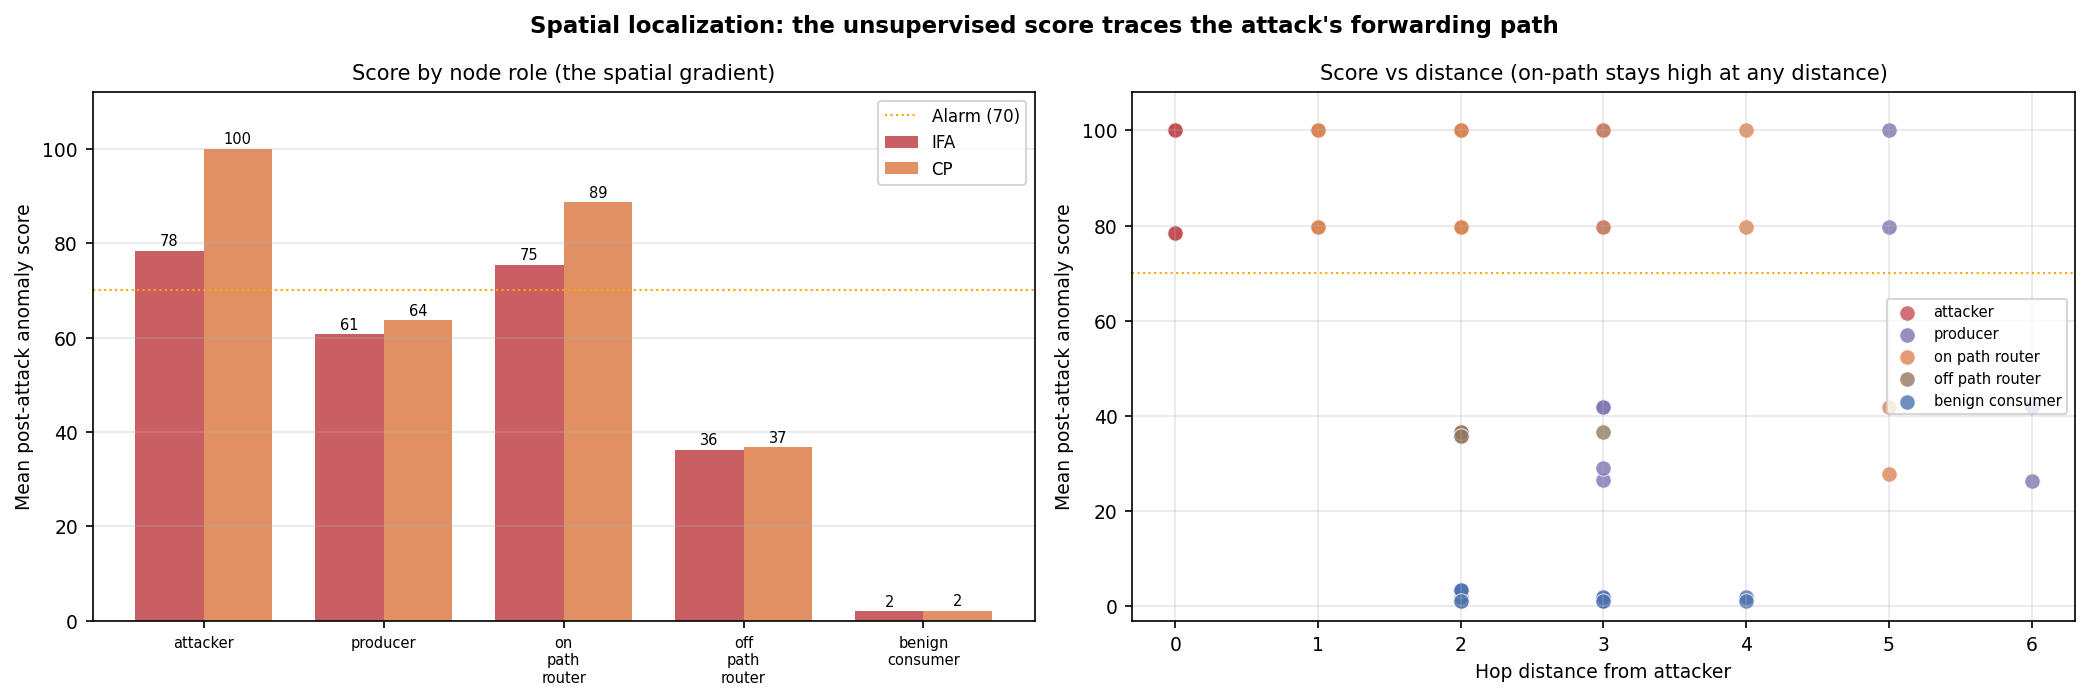
\includegraphics[width=0.85\textwidth]{fig_spatial_localization}
    \caption{Mean anomaly score by node role and score versus hop distance (ndnSIM). The score traces the attack's forwarding path rather than decaying with hop count.}
    \label{fig:sim_spatial}
\end{figure}

\subsection{The Detection Floor}
\label{sec:sim-floor}

At the rate examined above, both attacks are detected essentially perfectly, which is exactly why that rate is uninformative about how stealthy an attacker can afford to be. Applying the detection-floor definition of Equation~\ref{eq:floor} to every sweep point instead answers the question that matters: as the attacker throttles down toward the legitimate background, at what rate does detection stop being reliable? Table~\ref{tab:sim-floor} reports pooled attacker-node detection against rate, aggregated over all three topologies and every replicate seed.

\begin{table}[t]
\centering
\caption{ndnSIM attacker-node detection (\%) versus rate, pooled over topologies and seeds. ``--'' means the rate was not sampled for that attack.}
\label{tab:sim-floor}
\begin{tabular}{@{}lcccccccccc@{}}
\toprule
\textbf{Rate (Hz)} & 1 & 2 & 10 & 20 & 30 & 35 & 40 & 45 & 50 & 100 \\
\midrule
\textbf{CP}  & -- & -- & 21 & 42 & 60 & 71 & 83 & 92 & 100 & 100 \\
\textbf{IFA} & 60 & 99.9 & 100 & 100 & 100 & -- & -- & -- & 100 & 100 \\
\bottomrule
\end{tabular}
\end{table}

The two curves in Table~\ref{tab:sim-floor} do not fail in the same way. \textbf{CP degrades gracefully}: detection falls from saturation at 50\,Hz and above down through 92\,\% at 45\,Hz, 83\,\% at 40\,Hz, 71\,\% at 35\,Hz, and 60\,\% at 30\,Hz, to about 21\,\% at 10\,Hz, tracking the attacker's rate smoothly the whole way down. Its 90\,\% crossing lands in the 40--45\,Hz band that was swept, at approximately \textbf{44\,Hz}. That gradual slope is itself informative: because CP's only signature is added request volume, its detectability is a function of how far above the legitimate background the attacker's rate sits, and as that rate approaches the background it simply sinks into it. \textbf{IFA fails almost nowhere in the range sampled}: detection holds at 100\,\% at every rate from 2\,Hz up through 100\,Hz, and only collapses to 60\,\% at 1\,Hz. Interpolating that near-vertical drop places IFA's 90\,\% crossing in the 1--2\,Hz band, at approximately \textbf{1.8\,Hz}, roughly the volume a single legitimate consumer produces. The two floors are an order of magnitude apart, and Figure~\ref{fig:floor-headline} puts them on the same axis: CP's floor sits at the high end of the swept range, IFA's at the low end, with the dashed 90\,\% line separating reliable detection from chance for each attack in a visibly different place.

\begin{figure}[t]
    \centering
    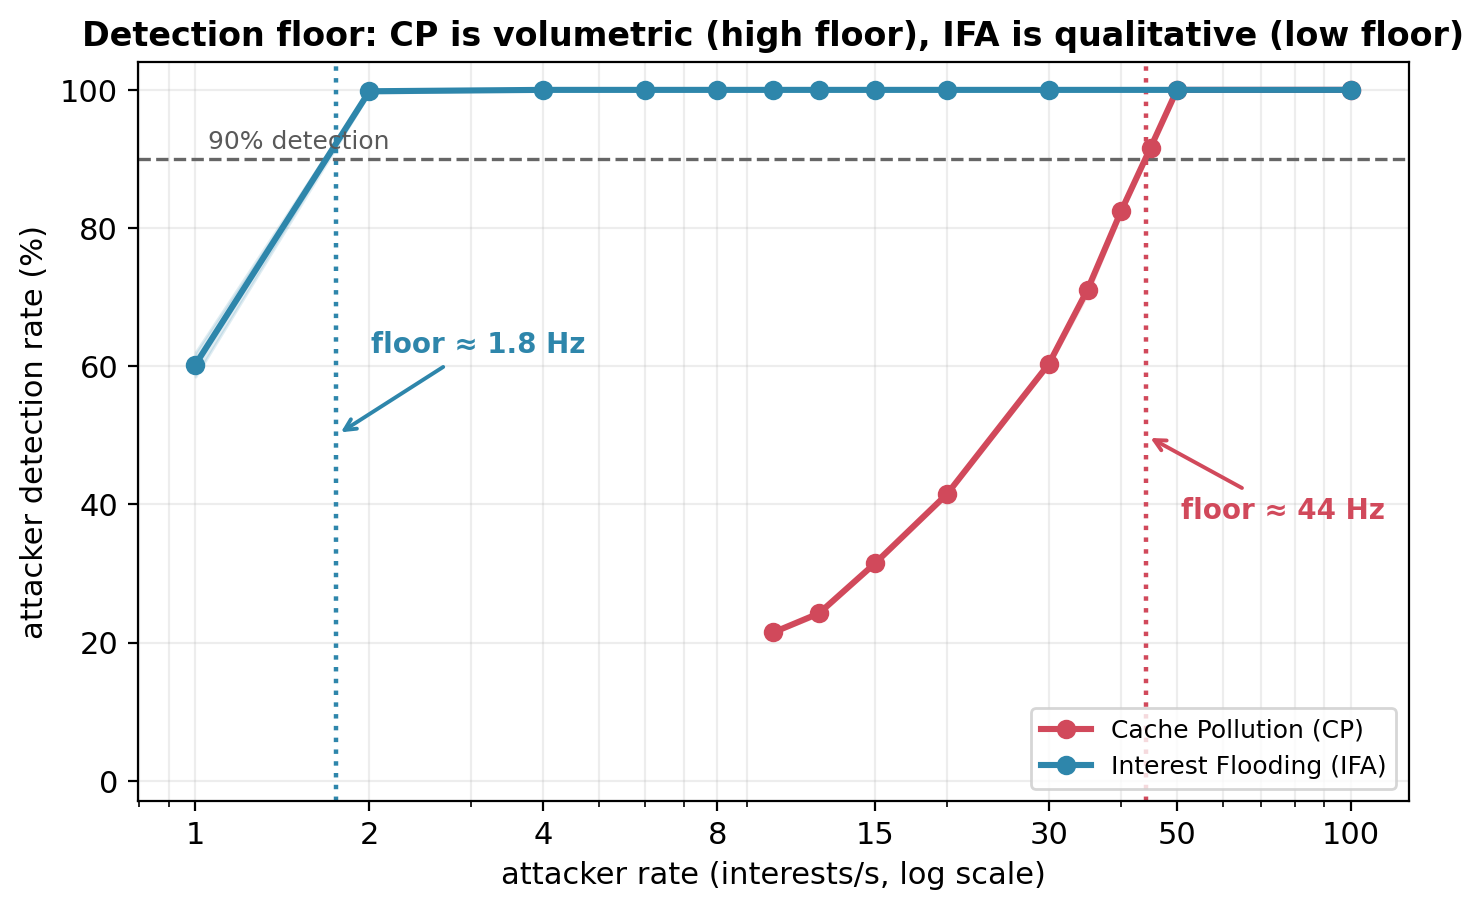
\includegraphics[width=0.74\textwidth]{fig_floor_headline}
    \caption{ndnSIM detection floor against live traffic. CP (volumetric) has a high floor (about 44\,Hz); IFA (qualitative timeout/NACK signature) has a floor an order of magnitude lower (about 1.8\,Hz). Shaded bands are $\pm 1$\,SD over topologies and seeds; the dashed line marks 90\,\% detection.}
    \label{fig:floor-headline}
\end{figure}

Two caveats bound how the floor numbers above should be read. First, the two highest rates swept for each attack, 50\,Hz and 100\,Hz, are single-seed anchors rather than five-seed averages; they confirm that detection stays saturated well above the floor but should not be read with the same statistical weight as the floor-region points. Second, a floor measured against an idle network would be meaningless, since an idle background gives a trivial 0\,\% false-positive rate and inflates any apparent floor; every number in Table~\ref{tab:sim-floor} is instead measured against the live traffic established earlier in this section, at a realistic false-positive rate of 1--2\,\% on clean traffic (about 0.8--1.0\,\% in the tree and DFN topologies, about 2\,\% in the dumbbell), so the floor reflects a genuine operating limit rather than an artifact of a silent network.

Neither floor is an accident of one network's shape. Figure~\ref{fig:detection-floor} breaks the same sweep out per topology, with per-seed spread shown alongside each curve, and the three topology curves are essentially superimposed for both attacks: the floor is a property of the attack's mechanism, not of whether the network is a tree, a dumbbell, or a mesh. That the two floors sit an order of magnitude apart, and that each holds regardless of topology, is the central quantitative result of this paper. Why they differ by that much, and specifically why CP's signature washes out gradually while IFA's holds until it nearly disappears, is a question about mechanism rather than measurement, and it is taken up directly in the next section.

\begin{figure}[t]
    \centering
    
\includegraphics[width=0.9\textwidth]{fig_detection_floor}
    \caption{Detection floor per topology (CP left, IFA right) with per-seed spread. The three topology curves are essentially superimposed and the per-seed spread is tight, so the floor is reproducible and topology-independent.}
    \label{fig:detection-floor}
\end{figure}

% Mechanism — drafted in Task N

% Discussion
\section{Discussion}
\label{sec:discussion}

\subsection{Security Implication of the Floor Gap}

The result that matters for an operator is not how well either attack is detected at a rate the attacker would never choose, but how far each attacker can throttle down before detection stops being reliable. Section~\ref{sec:simulation} located that point directly: CP's 90\,\% crossing sits at roughly 44\,Hz, IFA's at roughly 1.8\,Hz, an order of magnitude apart, and Section~\ref{sec:mechanism} showed the gap is a property of what each attack is rather than of the network it runs over. Read as a bound on attacker behaviour rather than as a detector score, this says something asymmetric about the two threats. An IFA attacker can throttle down almost to the rate a single ordinary consumer already produces and still remain invisible, because a broken outcome is a broken outcome regardless of how rarely it occurs; there is close to no headroom between ``attacking'' and ``blending in.'' A CP attacker has no such option: to stay under the floor it must also stay under roughly the legitimate background's own volume, which caps how much cache damage it can do while quiet and forces it to choose between being loud and being effective. CP is therefore the easier attack to catch behaviorally, precisely because its only lever, added volume, is also its only liability. IFA is the more dangerous stealth threat of the two, not because it is harder to detect at any given rate, Table~\ref{tab:sim-floor} shows the opposite, but because the rate at which it stops being detectable is so close to the rate at which it stops being an attack at all. Crucially, this floor is measured against a realistic operating point rather than an idealized one: as Figure~\ref{fig:fpr} shows, the benign-consumer false-positive rate stays flat at a realistic 1--2\,\% across the swept attacker rates, rather than the trivial 0\,\% an idle network would give, so the floor reflects a genuine detection limit and not an artifact of a silent baseline.

\begin{figure}[t]
    \centering
    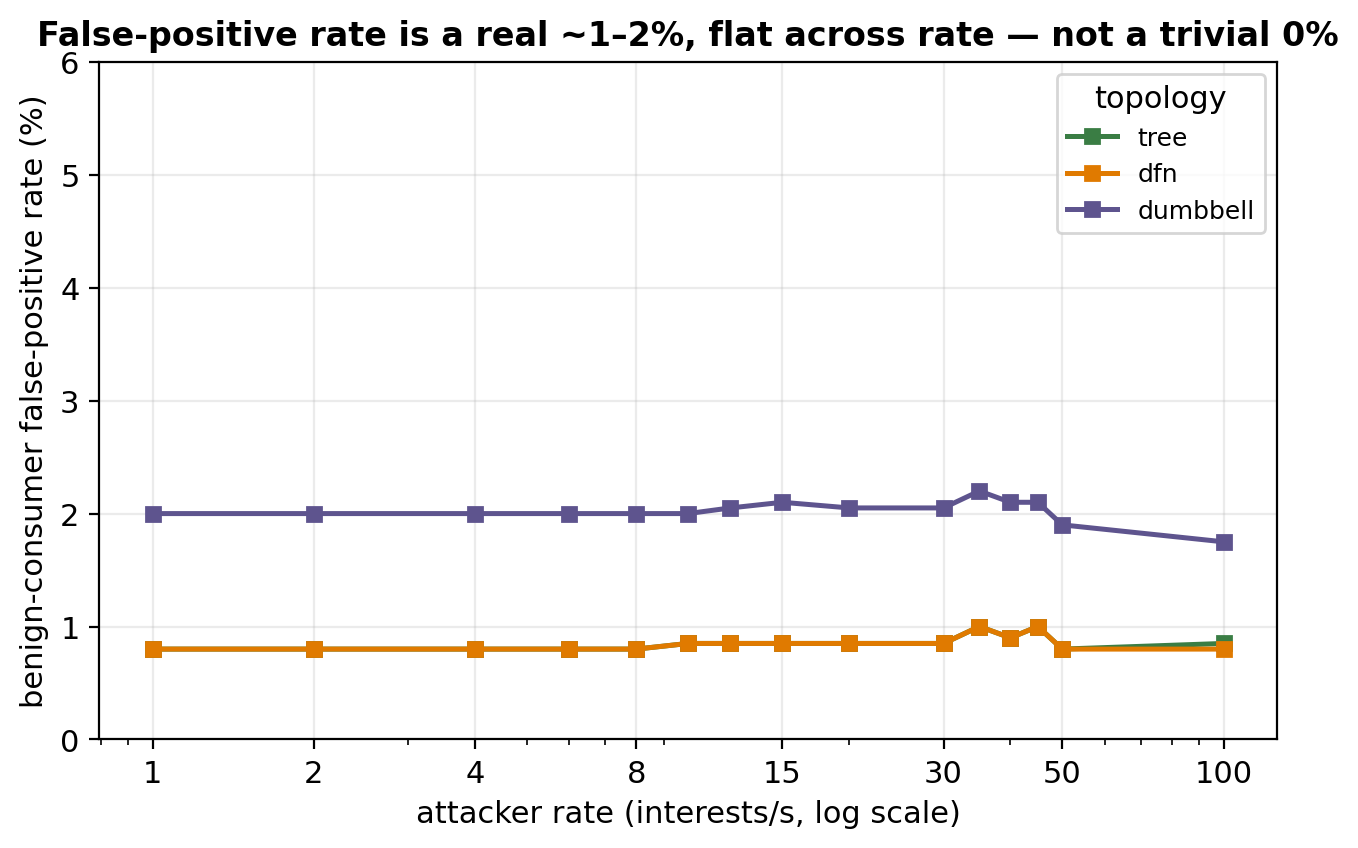
\includegraphics[width=0.7\textwidth]{fig_fpr_vs_rate}
    \caption{Benign-consumer false-positive rate against live traffic, swept across attacker rates. The rate stays a flat, realistic 1--2\,\%, rather than the trivial 0\,\% an idle network would produce.}
    \label{fig:fpr}
\end{figure}

\subsection{Comparison with Rule-Based Detection}

A conventional NDN security posture applies static thresholds to a handful of counters, typically interest rate, satisfaction ratio, PIT size, and NACK rate, and flags whichever counter crosses its line. Such a detector is structurally blind to Cache Pollution: CP's requests are answered, so satisfaction ratio, the metric most commonly monitored, stays high throughout the attack, and the only thing CP disturbs is a cache-hit ratio that a single-threshold rule rarely watches at all. The same detector is also weakened on its own home ground, IFA, by leaning on PIT size, which Section~\ref{sec:emulation} showed is non-discriminating once polling happens on a realistic multi-second interval rather than continuously. A rule-based detector's failure mode is therefore not narrow; it misses CP because it watches the wrong feature and misses IFA because the feature it does watch has already washed out by the time it is read. The Isolation Forest used throughout this paper does not need any single feature to cross a line, because it scores the joint improbability of the whole feature vector: a low cache-hit ratio co-occurring with otherwise ordinary traffic, or a collapsed satisfaction ratio alongside a normal-looking request rate, is exactly the kind of improbable combination a multi-feature model recognises and a single threshold cannot.

\subsection{Cross-Platform Consistency}

The floor result would carry less weight if it depended on one simulator's traffic model or one topology's geometry. It does not. On the emulation platform, Section~\ref{sec:method}'s global model, trained once across all three topologies, matches or beats per-topology models, and the same path-localised anomaly pattern, attacker and on-path nodes flagged, off-path nodes near baseline, is independently reproduced on both platforms: on miniNDN's real forwarding daemon (Section~\ref{sec:emulation}) and on ndnSIM's simulator (Section~\ref{sec:simulation}). Two platforms built on different codebases, one running actual NFD binaries under emulation and the other an ns-3 discrete-event model, reproducing the same qualitative behaviour is stronger evidence than either platform could offer alone; it suggests the pattern reflects how IFA propagates through NDN forwarding rather than an artifact of one simulator's approximations.

\subsection{A Note on Deployment}

To confirm the detector is usable outside a labelled offline evaluation, a real-time monitoring implementation, a live per-node scoring dashboard, was built and used to demonstrate the detector operating online; its architecture is outside this paper's scope.

\subsection{Limitations and Future Work}

Several limitations bound how these results should be read. The emulation track covers IFA only; CP required an active cache to leave a footprint at all (Section~\ref{sec:simulation}), so its evaluation rests entirely on simulation, and the two attacks were never run concurrently on either platform. miniNDN's 3\,s polling interval averages out sub-second PIT dynamics, which is the direct explanation for why \textit{pit\_size} and \textit{pit\_growth\_rate} proved non-discriminating in Section~\ref{sec:emulation} rather than evidence that PIT state is uninformative in principle; sub-second polling is a natural next step to test whether it recovers a usable PIT signal. The floor crossings reported in Section~\ref{sec:simulation} are interpolated between sampled rates rather than measured at the exact crossing point, so they are best read as bands, CP 40--45\,Hz, IFA 1--2\,Hz, and the two highest swept rates for each attack rest on a single seed rather than the five-seed average used in the floor region. The Isolation Forest deployed here is static: it does not adapt to gradual concept drift in legitimate traffic and would need periodic retraining in a long-running deployment. IFA's floor is set by traffic mimicry, the attacker leaves almost nothing outside the timeout and NACK ratios for the detector to work with, and augmenting the feature set with temporal statistics, for example autocorrelation of the NACK rate or of inter-arrival times, is a plausible route to pushing that floor lower still. Finally, none of this addresses content-integrity attacks that preserve normal traffic statistics while serving corrupted data; those attacks leave no behavioral trace for this kind of detector to find and would need complementary signature or provenance verification rather than anomaly detection.

% Conclusion
\section{Conclusion}
\label{sec:conclusion}

This paper presented a single unsupervised Isolation Forest detector, trained only on clean traffic, evaluated on two independent NDN platforms, miniNDN's emulation of the real NDN Forwarding Daemon and the ndnSIM simulator, across the same three topologies. One detector, one training regime, no labelled attack data: the design was deliberately shared end to end so that differences in outcome could be attributed to the attacks and the platforms rather than to inconsistent methodology.

The emulation study corrects the conventional picture of the Interest Flooding Attack. The global model identifies the attacker node at 91.2--98.7\,\% across the three topologies at a false-positive rate below 4.3\,\%, but PIT-based features, the textbook signature of IFA, turn out to be non-discriminating at practical polling intervals; satisfaction ratio, cache-hit ratio, and NACK rate carry the signal instead. Cache Pollution leaves no usable footprint in this feature set, a negative result that motivated the simulation study.

The simulation study supplies the paper's central finding. An attacker-rate sweep locates two detection floors that are an order of magnitude apart and topology-invariant: Cache Pollution, a volumetric attack, remains reliably detectable down to roughly 44\,Hz, while Interest Flooding, whose signature is qualitative rather than volumetric, remains detectable down to roughly 1.8\,Hz, both at a realistic 1--2\,\% false-positive rate. The gap is mechanistic rather than incidental: a purely volumetric attack cannot hide below the legitimate background rate without ceasing to be effective, while a qualitative attack can throttle down close to that rate and still remain invisible.

Taken together, these results indicate that the security-relevant limit on unsupervised NDN anomaly detection is not peak detection accuracy at a single, easily separable attack rate, but the mechanism-dependent floor below which an attacker can operate undetected. Reporting a floor rather than a peak reframes what a detector's evaluation should answer: not whether the attack can be caught, but how quiet the attacker can be before it stops being caught. This distinction is what future work on stealthier variants of both attacks, and on complementary detection strategies for content-integrity threats, should be measured against.

% Declarations — drafted in Task N


\bibliographystyle{unsrtnat}
\bibliography{references}

\end{document}
